%!TEX encoding = UTF-8 Unicode
\documentclass[a4paper,UTF8,heading=false,12pt]{article}
\usepackage[heading = false]{ctex}
\usepackage{graphicx}

% package
\usepackage{xeCJK}
\usepackage{blindtext}
\usepackage{palatino}
% \usepackage{titlesec}
\usepackage{needspace}
\usepackage[toc,page]{appendix}
\usepackage{metainfo}
\usepackage[pagestyles,raggedright]{titlesec}
\usepackage[xetex,colorlinks=false,hidelinks,pdfstartview=FitV]{hyperref}
\usepackage{amsmath,amssymb}
\usepackage{newpxtext,newpxmath}
\usepackage{listings}
\usepackage{fontspec}
\usepackage{xcolor-material}
\usepackage{enumitem}
\usepackage{booktabs}
\usepackage{multicol}
% configuration
\fontsize{16pt}{\baselineskip}
\setmonofont{FiraCode Nerd Font}
\CJKfamily{zhsong}
%\addtolength{\parindent}{3cm}
% code configuration
\definecolor{codegreen}{rgb}{0,0.6,0}
\definecolor{codegray}{rgb}{0.5,0.5,0.5}
\definecolor{codepurple}{rgb}{0.58,0,0.82}
\definecolor{backcolour}{rgb}{0.95,0.95,0.92}
\lstdefinestyle{customc}{
    belowcaptionskip=1\baselineskip,
    breaklines=true,
    frame=none,
    xleftmargin=2em,
    language=C++,
    showstringspaces=false,
    basicstyle=\footnotesize\ttfamily,
    keywordstyle=\bfseries\color{green!40!black},
    commentstyle=\itshape\color{purple!40!black},
    numberstyle=\fontspec{FiraCode Nerd Font}\color{darkgray},
    numbers=left,
    identifierstyle=\color{blue},
    stringstyle=\color{orange},
}

\usepackage[paperwidth=210mm, paperheight=297mm, margin=20 mm]{geometry}

\newcommand\subtitle[1]{{\small #1}} 
\renewcommand{\normalsize}{\fontsize{12}{12}\selectfont}
\begin{document}
    \title{
        数据库系统概论实验报告 \\
        \subtitle{实验三: 使用两种方式操作数据表}
    }
    \author{陈羿羽 \thanks{陈羿羽:西南大学2019级计算机科学与技术4班 - 222019603193014}}
    \maketitle

    \begin{abstract}
        本次实验的目标为:
        \begin{enumerate}
            \item 使用数据库管理系SQL Server 或者MySQL操作数据库。
            \item 掌握创建、查看、修改和删除数据表的基本操作。
        \end{enumerate}
    \end{abstract}

    \newpage

    \section{实验准备}

    \begin{enumerate}
        \item 一台PC机或笔记本电脑
        \item 能够上网
    \end{enumerate}

    \section{实验要求}

    \begin{enumerate}
        \item 查资料观看数据库管理系SQL Server 或者MySQL的数据表操作视频。
        \item 使用视图方式和命令方式创建数据表、查看、修改和删除数据表。
        \item 学习了解数据表字段的基本类型。
    \end{enumerate}

    \section{实验内容}

    \subsection{视图方式建立数据表}
    向实验二以自己名字(拼音简写)创建一个数据库中添加下面结构的数据表。

    \subsubsection{学生成绩表格}

    实验要求的数据表如下表1所示。
    
    \begin{table}[htbp]
        \begin{center}
            \begin{tabular}{@{}ccccc@{}}
            \toprule
            序号 & 字段名  & 字段类型     & 宽度 & 可否为空 \\ \midrule
            1  & 学号   & nvarchar & 10 & 否    \\
            2  & 姓名   & nvarchar & 8  & 否    \\
            3  & 班级   & nvarchar & 20 & 否    \\
            4  & 学期   & nvarchar & 50 & 否    \\
            5  & 课程名称 & nvarchar & 20 & 否    \\
            6  & 分数   & nvarchar &    &      \\ \bottomrule
            \end{tabular}
            \caption{实验要求的学生成绩表}
        \end{center}
    \end{table}

    由于这个表是Oracle的表,部分内容不兼容Mysql,同时有部分内容与接下来的表一致性上有冲突,所以此处做出了修改,如下表2所示。

    \begin{table}[htbp]
        \begin{center}
            \begin{tabular}{@{}cccccc@{}}
                \toprule
                序号 & 字段名         & 字段类型    & 宽度  & 可否为空 & 备注   \\ \midrule
                1  & StudentId   & integer & 10  & 否    & 学号   \\
                2  & StudentName & varchar & 255 & 否    & 姓名   \\
                3  & ClassId     & integer & 20  & 否    & 班级   \\
                4  & TermId      & integer & 50  & 否    & 学期   \\
                5  & CourseName  & varchar & 255 & 否    & 课程名称 \\
                6  & Score       & decimal & 20  &      & 分数   \\ \bottomrule
                \end{tabular}
                \caption{修改适配后的学生成绩表}
        \end{center}
    \end{table}

    使用DataGrip创建学生成绩表的过程如下图1所示。

    \begin{figure}[htbp]
        \centering
        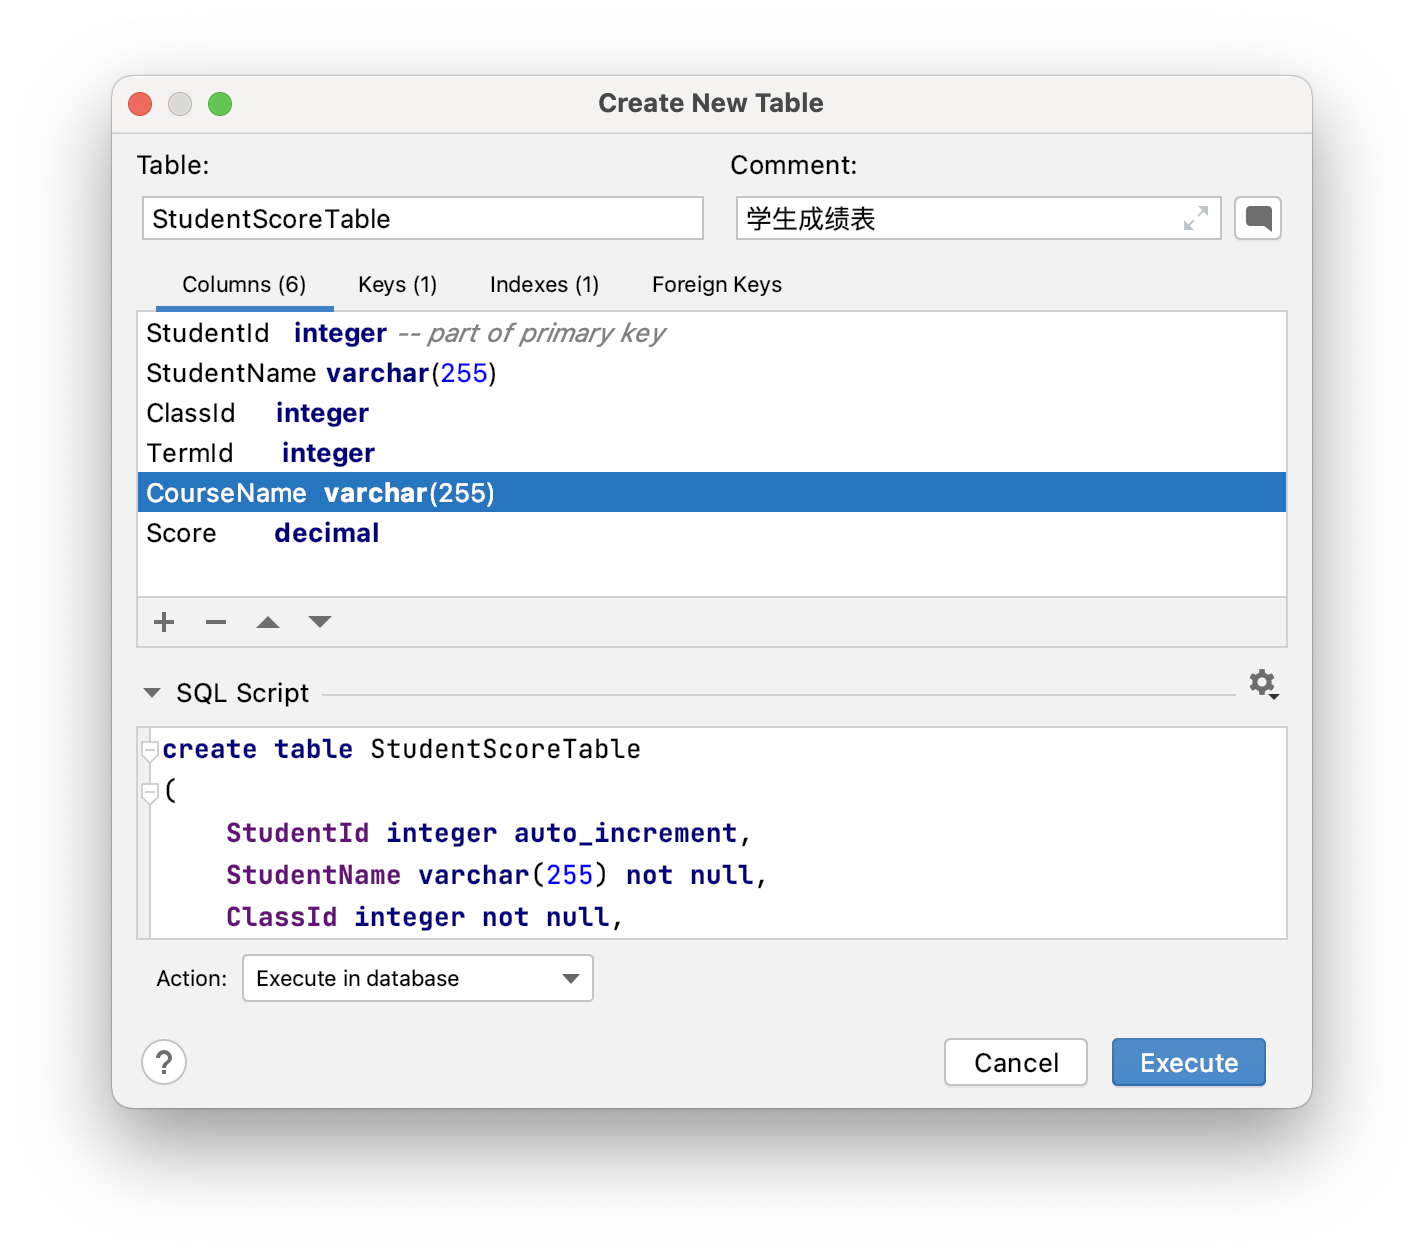
\includegraphics[width=10cm]{../Images/StudentScoreTable.png}
        \caption{使用DataGrip的视图创建学生成绩表}
    \end{figure}

    \subsubsection{班级信息表格}

    实验要求的班级信息表格如下表3所示。

    \begin{table}[htbp]
        \begin{center}
            \begin{tabular}{@{}ccccc@{}}
            \toprule
            序号 & 字段名  & 字段类型     & 宽度 & 可否为空 \\ \midrule
            1  & 班级   & nvarchar & 16 & 否    \\
            2  & 年级   & nvarchar & 16 & 否    \\
            3  & 专业   & nvarchar & 16 & 否    \\
            4  & 人数   & nvarchar & 8  & 否    \\
            5  & 教师   & nvarchar & 5  & 否    \\
            6  & 班主任   & nvarchar & 8 & 否   \\ \bottomrule
            \end{tabular}
            \caption{实验要求的班级信息表格}
        \end{center}
    \end{table}

    由于这个表是Oracle的表,部分内容不兼容Mysql,同时有部分内容与上下文的表一致性上有冲突,所以此处做出了修改,如下表4所示。

    \begin{table}[htbp]
        \begin{center}
            \begin{tabular}{@{}cccccc@{}}
                \toprule
                序号 & 字段名         & 字段类型    & 宽度  & 可否为空 & 备注   \\ \midrule
                1  & ClassId   & integer & 20  & 否    & 班级   \\
                2  & GradeId & integer & 20 & 否    & 年级   \\
                3  & MajorName     & varchar & 255  & 否    & 专业名称   \\
                4  & StudentCount & integer & 20  & 否    & 班级人数   \\
                5  & TeacherName  & varchar & 255 & 否    & 教师名字 \\
                6  & MasterName & varchar & 255  & 否   & 班主任名字   \\ \bottomrule
                \end{tabular}
                \caption{修改适配后的班级信息表}
        \end{center}
    \end{table}

    使用DataGrip创建班级信息表的过程如下图2所示。

    \begin{figure}[htbp]
        \centering
        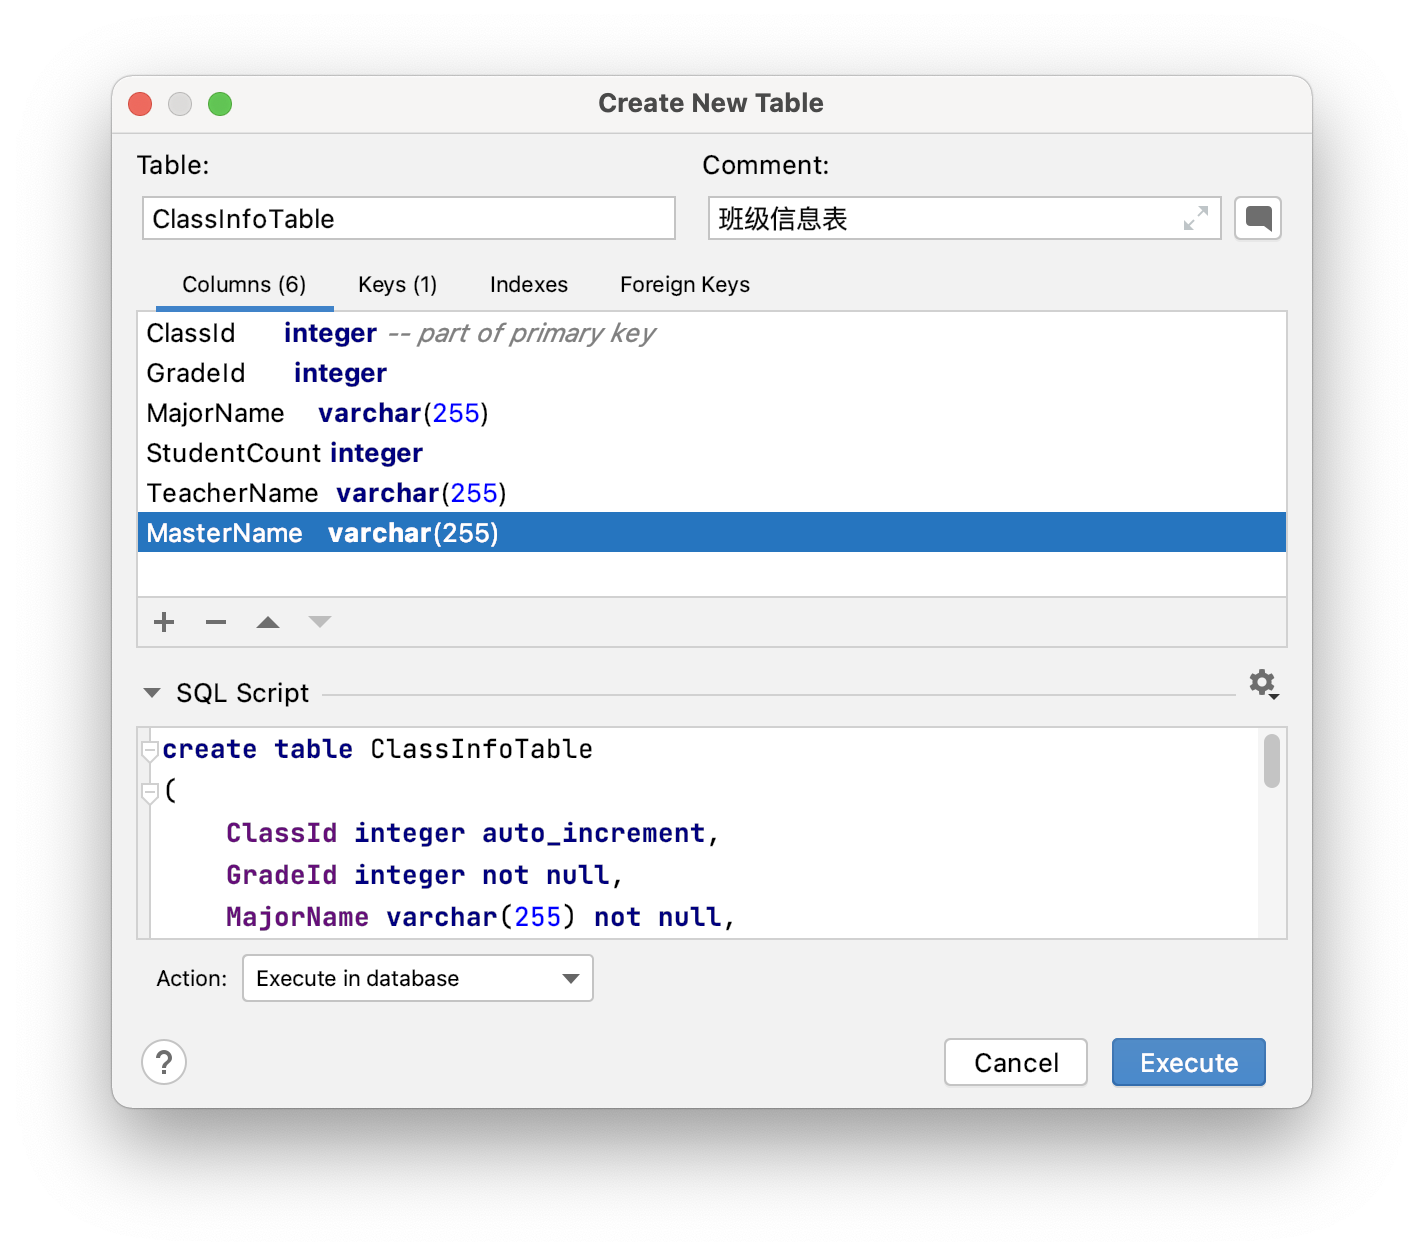
\includegraphics[width=10cm]{../Images/ClassInfoTable.png}
        \caption{使用DataGrip的视图创建班级信息表}
    \end{figure}

    \subsubsection{课程信息表格}

    实验要求的课程信息表格如下表5所示。

    \begin{table}[htbp]
        \begin{center}
            \begin{tabular}{@{}ccccc@{}}
            \toprule
            序号 & 字段名  & 字段类型     & 宽度 & 可否为空 \\ \midrule
            1  & 课程代码   & nvarchar & 20 & 否    \\
            2  & 课程名称   & nvarchar & 20 & 否    \\
            3  & 任课教师   & nvarchar & 20 & 否    \\\bottomrule
            \end{tabular}
            \caption{实验要求的课程信息表格}
        \end{center}
    \end{table}

    由于这个表是Oracle的表,部分内容不兼容Mysql,同时有部分内容与上下文的表一致性上有冲突,所以此处做出了修改,如下表6所示。

    \begin{table}[htbp]
        \begin{center}
            \begin{tabular}{@{}cccccc@{}}
                \toprule
                序号 & 字段名         & 字段类型    & 宽度  & 可否为空 & 备注   \\ \midrule
                1  & CourseId   & integer & 20  & 否    & 课程代码   \\
                2  & CourseName & varchar & 255 & 否    & 课程名称   \\
                3  & TeacherName     & varchar & 255  & 否    & 任课教师   \\ \bottomrule
                \end{tabular}
                \caption{修改适配后的课程信息表}
        \end{center}
    \end{table}

    使用DataGrip创建课程信息表的过程如下图3所示。

    \begin{figure}[htbp]
        \centering
        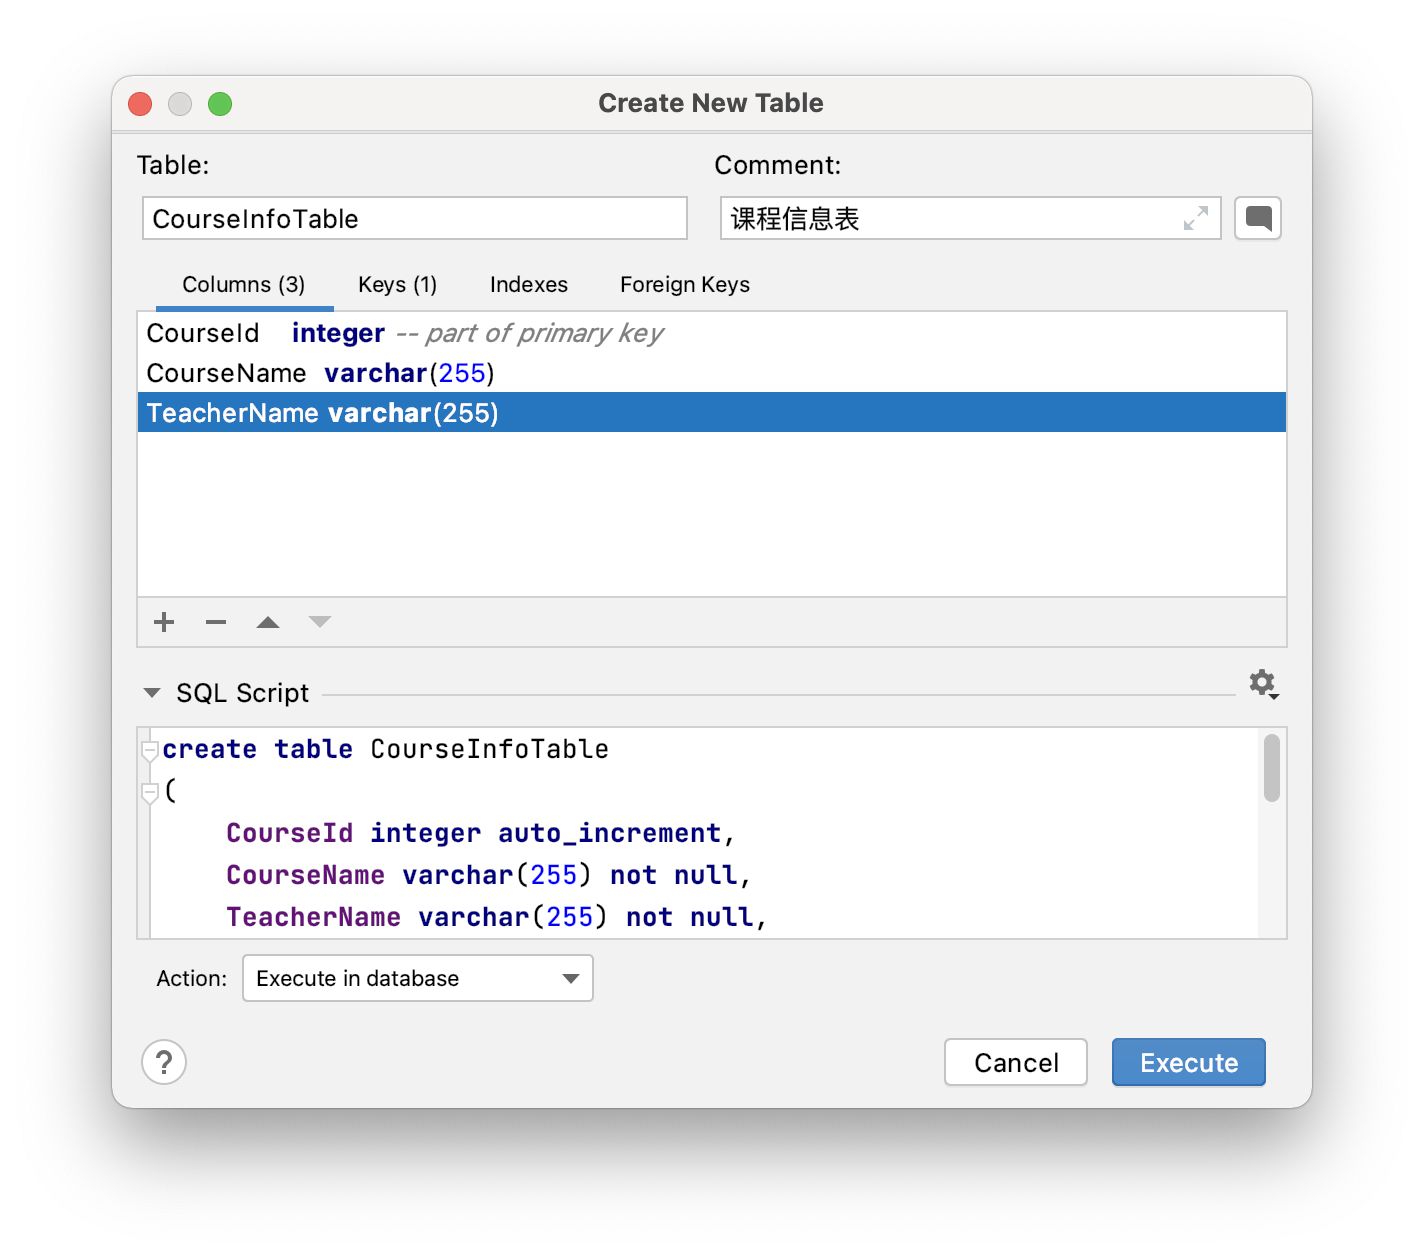
\includegraphics[width=10cm]{../Images/CourseInfoTable.png}
        \caption{使用DataGrip的视图创建课程信息表}
    \end{figure}

    \subsubsection{学生交费信息表格}

    实验要求的学生交费信息表格如下表7所示。

    \begin{table}[htbp]
        \begin{center}
            \begin{tabular}{@{}ccccc@{}}
            \toprule
            序号 & 字段名  & 字段类型     & 宽度 & 可否为空 \\ \midrule
            1  & 学号   & nvarchar & 5 & 否    \\
            2  & 学期   & nvarchar & 20 & 否    \\
            3  & 交费   & money & 20 & 否    \\
            4  & 欠费   & money & 20 & 否    \\
            5  & 日期   & smalldatetime & 20 & 否    \\
            \bottomrule
            \end{tabular}
            \caption{实验要求的学生交费信息表格}
        \end{center}
    \end{table}

    由于这个表是Oracle的表,部分内容不兼容Mysql,同时有部分内容与上下文的表一致性上有冲突,所以此处做出了修改,如下表8所示。

    \begin{table}[htbp]
        \begin{center}
            \begin{tabular}{@{}cccccc@{}}
                \toprule
                序号 & 字段名         & 字段类型    & 宽度  & 可否为空 & 备注   \\ \midrule
                1  & StudentId   & integer & 20  & 否    & 学号   \\
                2  & TermId & integer & 20 & 否    & 学期   \\
                3  & PaymentAmount     & decimal & 128  & 否    & 交费   \\ 
                4  & ArrearsAmount     & decimal & 128  & 否    & 欠费   \\ 
                5  & Date     & datetime & N/A  & 否    & 日期   \\ 
                \bottomrule
                \end{tabular}
                \caption{修改适配后的学生交费信息表}
        \end{center}
    \end{table}

    使用DataGrip创建课程信息表的过程如下图4所示。

    \begin{figure}[htbp]
        \centering
        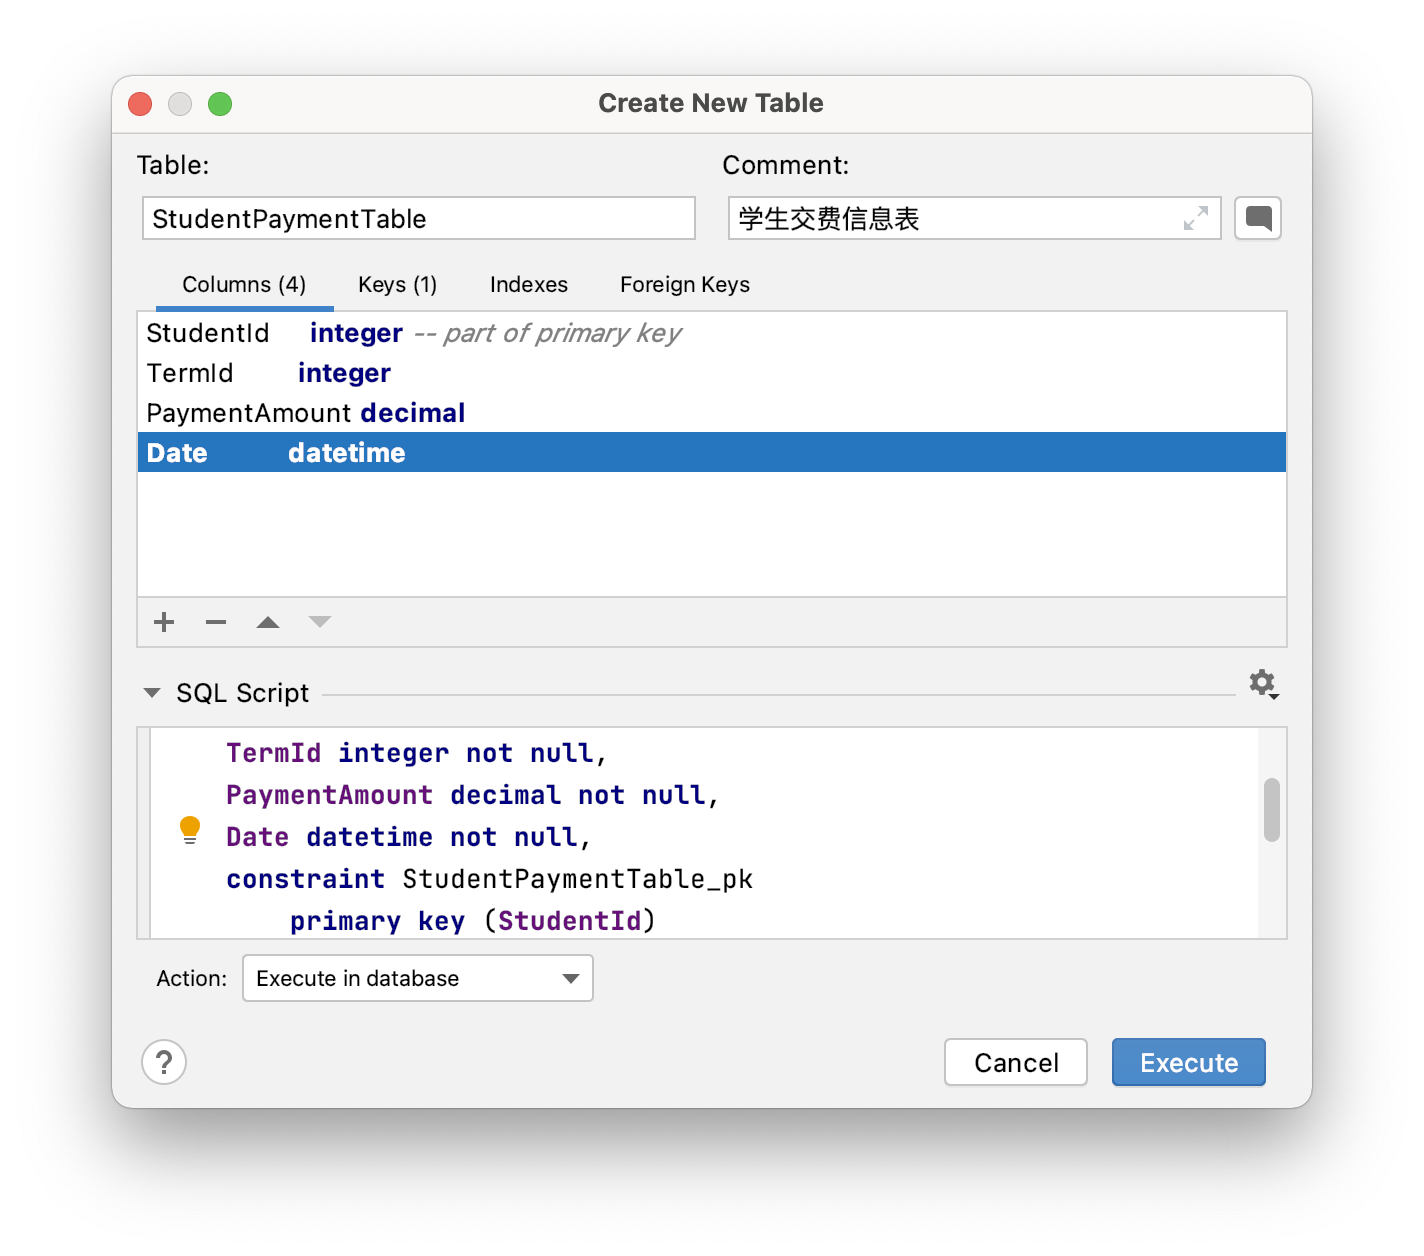
\includegraphics[width=10cm]{../Images/StudentPaymentTable.png}
        \caption{使用DataGrip的视图创建课程信息表}
    \end{figure}

    \subsubsection{学生学籍信息表格}

    实验要求的学生学籍信息表格如下表9所示\footnote{不知道为什么此处序号4重复了}。

    \begin{table}[htbp]
        \begin{center}
            \begin{tabular}{@{}ccccc@{}}
            \toprule
            序号 & 字段名  & 字段类型     & 宽度 & 可否为空 \\ \midrule
            1  & 学号   & nvarchar & 5 & 否    \\
            2  & 姓名   & nvarchar & 8 & 否    \\
            3  & 性别   & nvarchar & 2 & 否    \\
            4  & 年级   & nvarchar & 16 & 否    \\
            4  & 班级   & nvarchar & 10 & 否    \\
            5  & 出生年月   & smalldatetime & 20 & 否    \\
            6  & 家庭住址   & nvarchar & 30 & 否    \\
            7  & 邮政编码   & int & 20 & 否    \\
            8  & 联系   & int & 20 & 否    \\
            9  & 入学时间   & smalldatetime & 20 & 否    \\
            10  & 备注   & ntext & 20 & 否    \\
            \bottomrule
            \end{tabular}
            \caption{实验要求的学生学籍信息表格}
        \end{center}
    \end{table}

    由于这个表是Oracle的表,部分内容不兼容Mysql,同时有部分内容与上下文的表一致性上有冲突,所以此处做出了修改,如下表10所示。

    \begin{table}[htbp]
        \begin{center}
            \begin{tabular}{@{}cccccc@{}}
                \toprule
                序号 & 字段名         & 字段类型    & 宽度  & 可否为空 & 备注   \\ \midrule
                1  & StudentId   & integer & 20  & 否    & 学号   \\
                2  & StudentName & varchar & 255 & 否    & 姓名   \\
                3  & StudentSex  & bool & 1  & 否    & 性别   \\ 
                4  & GradeId     & integer & 20  & 否    & 年级   \\ 
                5  & ClassId     & integer & 20  & 否    & 班级   \\ 
                6  & StudentBirthday     & date & N/A  & 否    & 出生年月   \\ 
                7  & Address     & varchar & 255  & 否    & 家庭住址   \\ 
                8  & PostCode     & integer & 20  & 否    & 邮政编码   \\ 
                9  & ContactNumber     & varchar & 255  & 否    & 联系方式   \\ 
                10  & EnrollmentDate    & date & N/A  & 否    & 入学日期   \\ 
                11  & Comment    & varchar & 255  & 否    & 备注   \\ 
                \bottomrule
                \end{tabular}
                \caption{修改适配后的学生学籍信息表}
        \end{center}
    \end{table}

    使用DataGrip创建学生学籍信息表的过程如下图5所示。

    \begin{figure}[htbp]
        \centering
        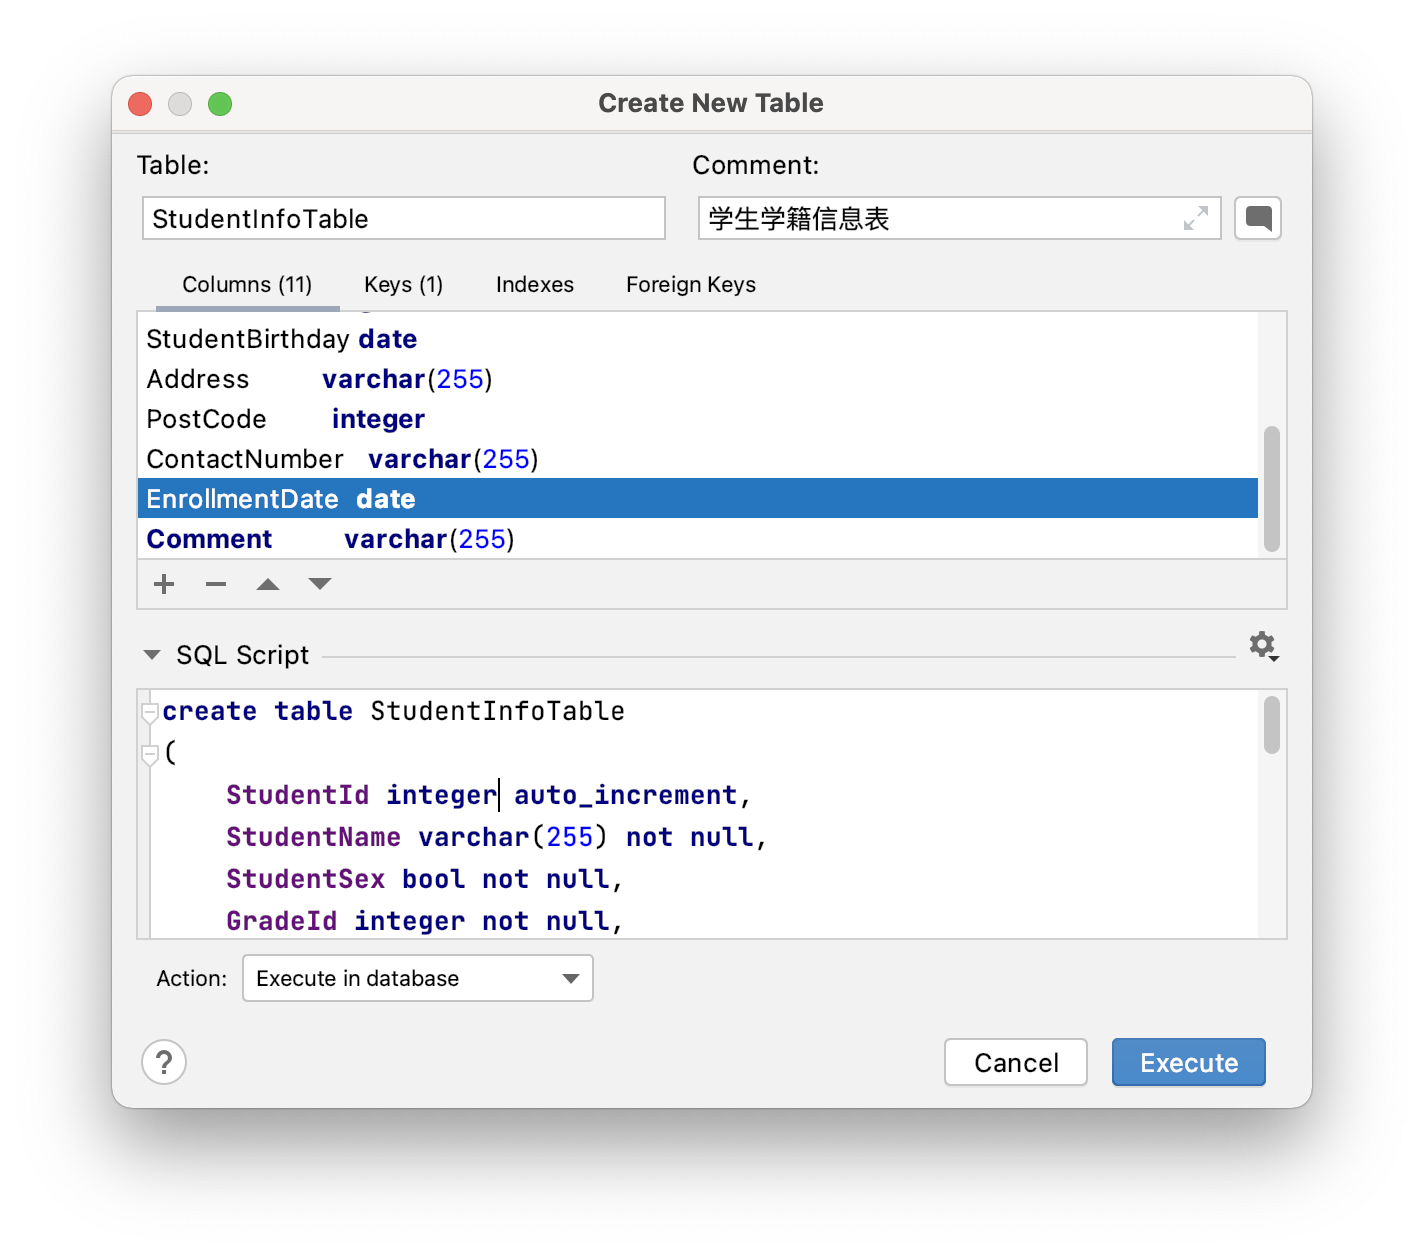
\includegraphics[width=10cm]{../Images/StudentInfoTable.png}
        \caption{使用DataGrip的视图创建课程信息表}
    \end{figure}

    \subsection{命令方式建立数据表}

    \subsection{使用视图方式和命令方式控制表}

    使用视图方式和命令方式添加test表、查看、修改(添加备注字段)和删除数据表test。实验要求的test表结构如下表`blocked`所示。

    \begin{table}[htbp]
        \begin{center}
            \begin{tabular}{@{}cccc@{}}
            \toprule
            字段名  & 字段类型  & 主键 & 说明 \\ \midrule
            ClsNo   & char(6) & 是 & 班号    \\
            ClsName & varchar(16) &  & 班名    \\
            Director & varchar(10) &  & 辅导员    \\
            Specialty   & varchar(30) &  & 专业    \\
            \bottomrule
            \end{tabular}
            \caption{实验要求的学生交费信息表格}
        \end{center}
    \end{table}

    \subsubsection{视图方式}

    我们先使用视图方式来创建test表,如下图`blocked`所示。

    \begin{figure}[htbp]
        \centering
        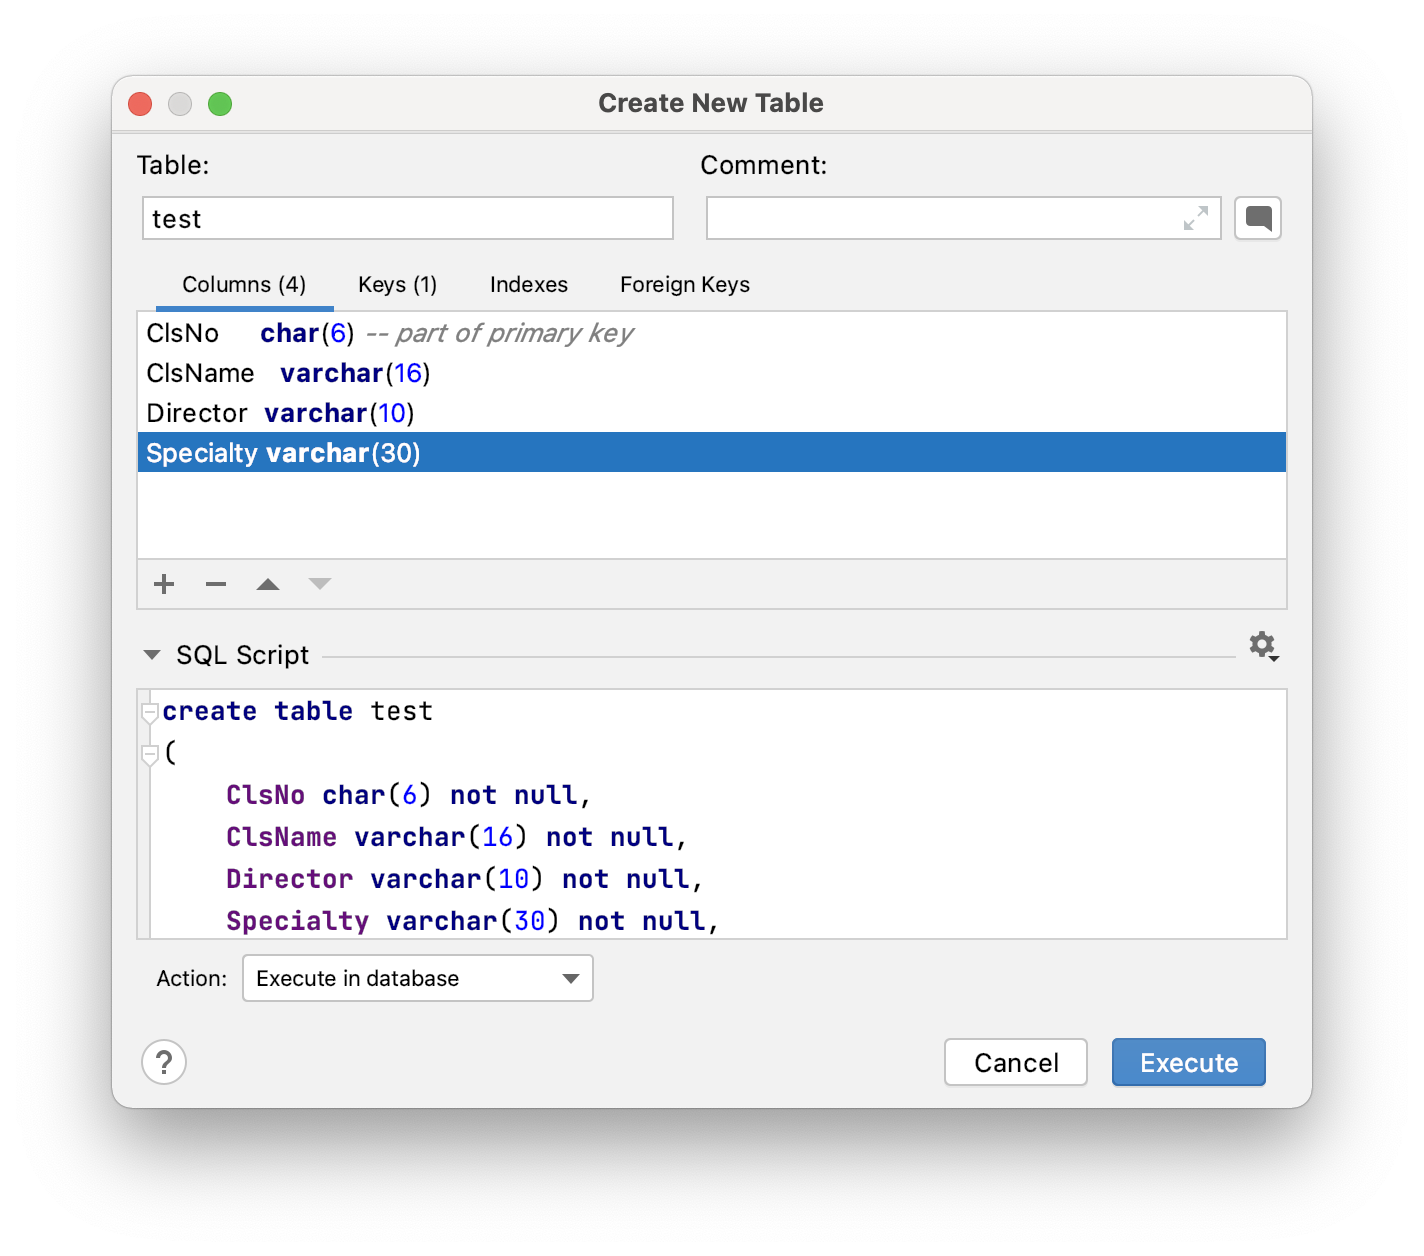
\includegraphics[width=10cm]{../Images/TestTable_OnCreate.png}
        \caption{使用DataGrip的视图创建test表}
    \end{figure}

    然后我们查看这个表,如下图`blocked`所示。

    \begin{figure}[htbp]
        \centering
        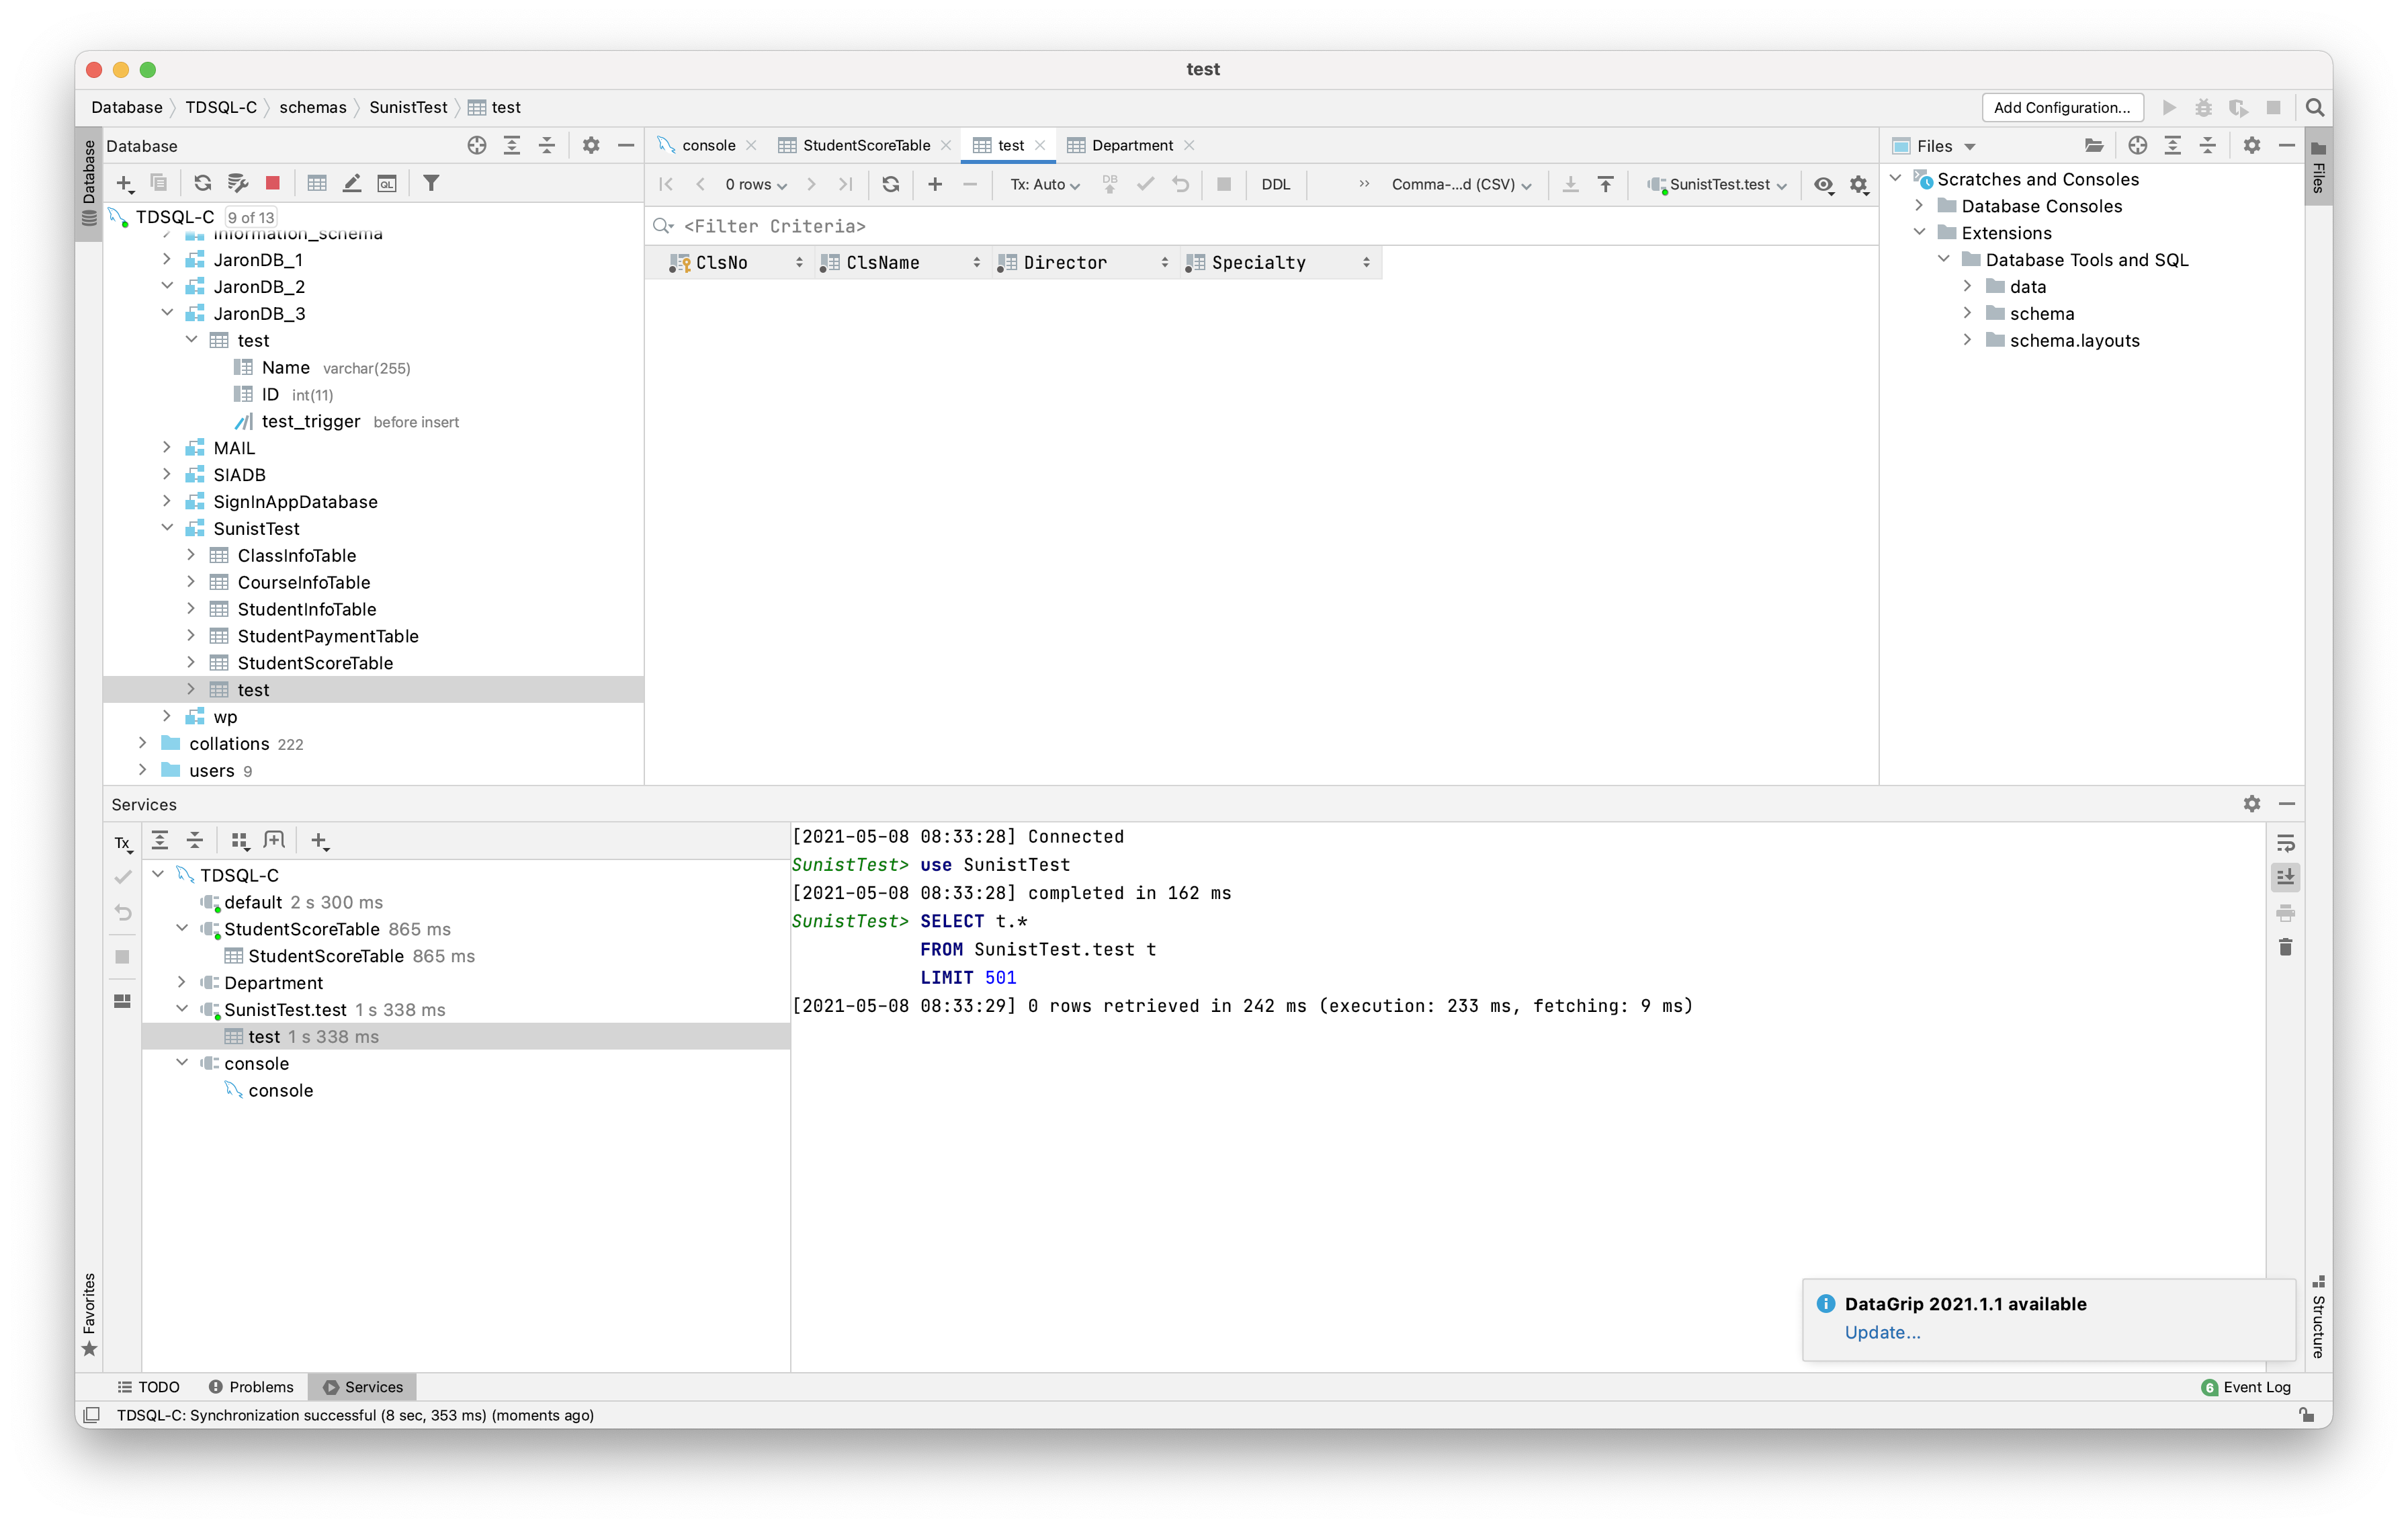
\includegraphics[width=15cm]{../Images/TestTable_OnView.png}
        \caption{使用DataGrip的视图浏览test表}
    \end{figure}

    然后我们修改这个表,添加Comment(varchar(255))字段,如下图`blocked`所示。

    \begin{figure}[htbp]
        \centering
        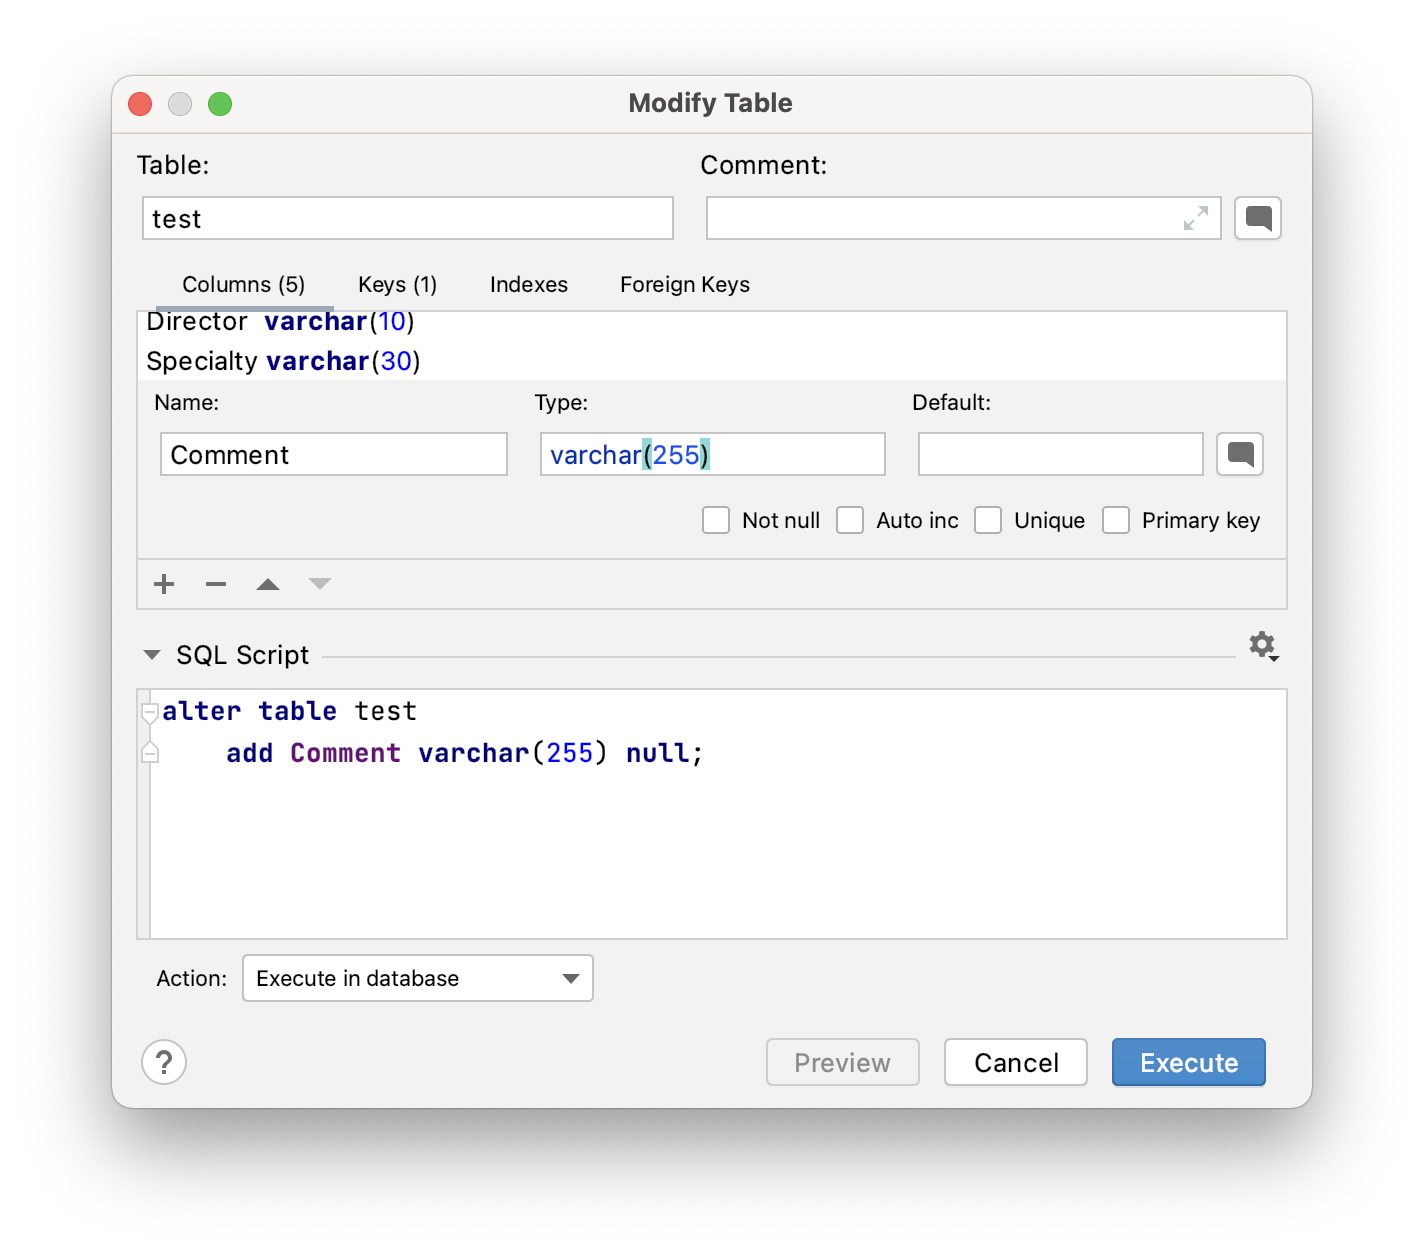
\includegraphics[width=10cm]{../Images/TestTable_OnChange.png}
        \caption{使用DataGrip的视图修改test表}
    \end{figure}

    最后我们删除这个表,如下图`blocked`所示。

    \begin{figure}[htbp]
        \centering
        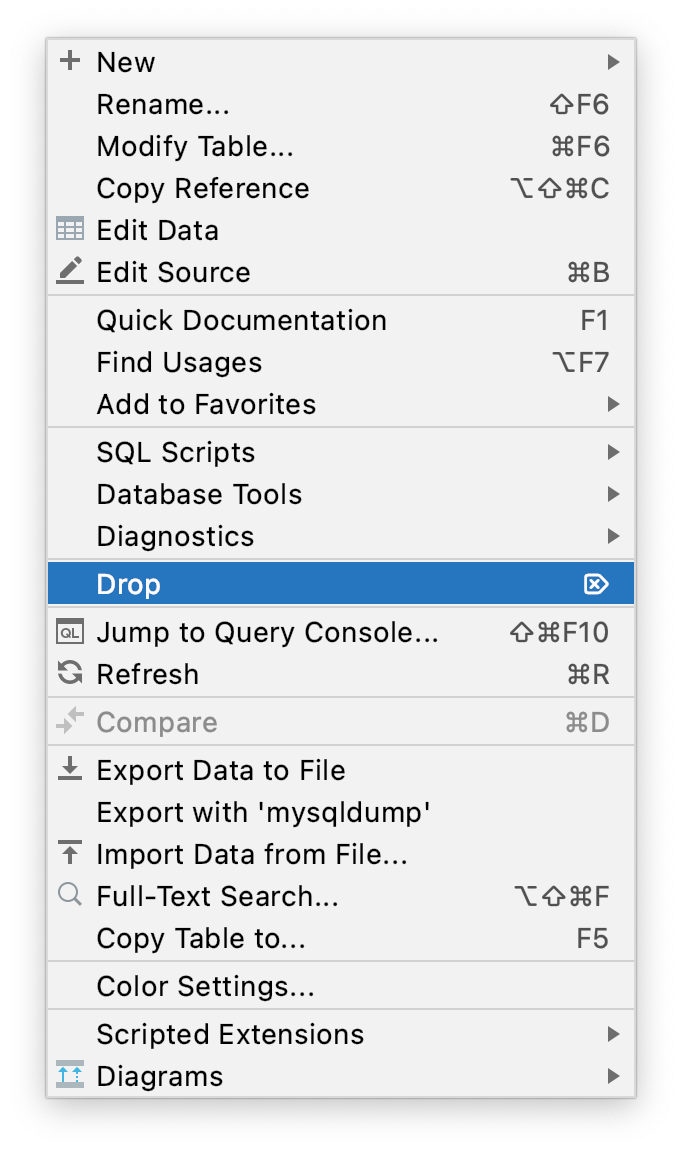
\includegraphics[width=10cm]{../Images/TestTable_OnDrop.png}
        \caption{使用DataGrip的视图删除test表}
    \end{figure}

    \subsubsection{命令方式}

    我们使用命令的方式操作test表,其步骤如下图`blocked`所示。

    \begin{figure}[htbp]
        \centering
        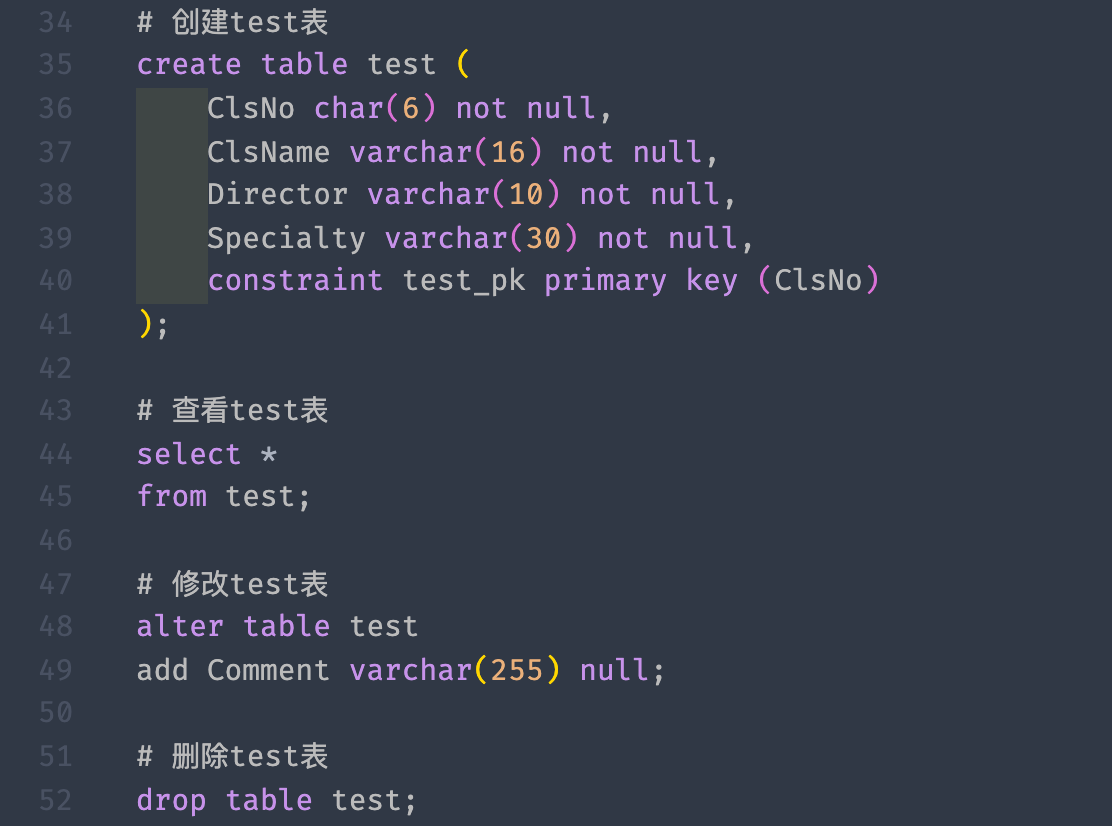
\includegraphics[width=15cm]{../Images/TestTable_WithCommand.png}
        \caption{使用命令行操作test表}
    \end{figure}

    \section{实验总结}

    \begin{enumerate}
        \item 设计合理数据表的重要性,设计时要考虑兼容性,像实验所要求的数据表在实际使用时基本无法使用,要尽量避免。
        \item DataGrip真好用。
    \end{enumerate}

\end{document}